\section{Εισαγωγή}

\subsection{Ταυτότητα - επιχειρησιακοί στόχοι}

Σκοπός της ομάδας saiko-killers είναι η δημιουργία μιας ενιαίας πλατφόρμας που ενθαρρύνει τη συνεργατική παρατήρηση τιμών πρατηρίων υγρών καυσίμων και παρέχει αυτές τις πληροφορίες δωρεάν σε κάθε χρήστη δίνοντας με αυτόν τον τρόπο έμμεσα τη δυνατότητα σε κάθε ιδιοκτήτη πρατηρίου υγρών καυσίμων να γνωρίζει τις τιμές στα ανταγωνιστικά πρατήρια υγρών καυσίμων και με βάση αυτές να καθορίζει την επιχειρηματική στρατιγική του.

\subsection{Περίγραμμα επιχειρησιακών λειτουργιών}

O ιδιοκτήτης πρατηρίου υγρών καυσίμων μετά την είσοδο στην ιστοσελίδα, το σύστημα ζητά τη συγκατάθεση του προκειμένου να λάβει τη γεωγραφική του τοποθεσία. \\
Ανεξάρτητα με το αν θα δώσει ή όχι τη συγκατάθεσή του θα μπορεί να πραγματοποιήσει αναζήτηση για τις τιμές καυσίμων με κριτήρια όπως θεματική ταξινόμηση, χρόνος και θέση.\\
Σε περίπτωση που δώσει τη συγκαταθεσή του, θα εμφανίζεται επιπρόσθετα στο χάρτη η τωρινή του τοποθεσία καθώς και τα πλησιέστερα σε αυτόν πρατήρια υγρών καυσίμων. Κάνοντας κλικ πάνω σε οποιοδήποτε απο αυτά του δίνεται η δυνατότητα να δει τις πλέον πρόσφατες τιμές καυσίμων για το συγκεκριμένο πρατήριο.\\
Με τις παραπάνω δυνατότητες ο ιδιοκτήτης πρατηρίου υγρών καυσίμων θα μπορεί να βλέπει πως κινούνται οι ανταγωνιστές του στην αγορά και με βάση αυτή την πληροφορία να κανονίζει την προσωπική του επιχειρηματική στρατηγική.\\
Η παραπάνω συμπεριφορά μοντελοποιείται με το διάγραμμα δραστηριοτήτων UML όμοιο με αυτο του χρήστη εθελοντή.

\begin{figure}
	\centering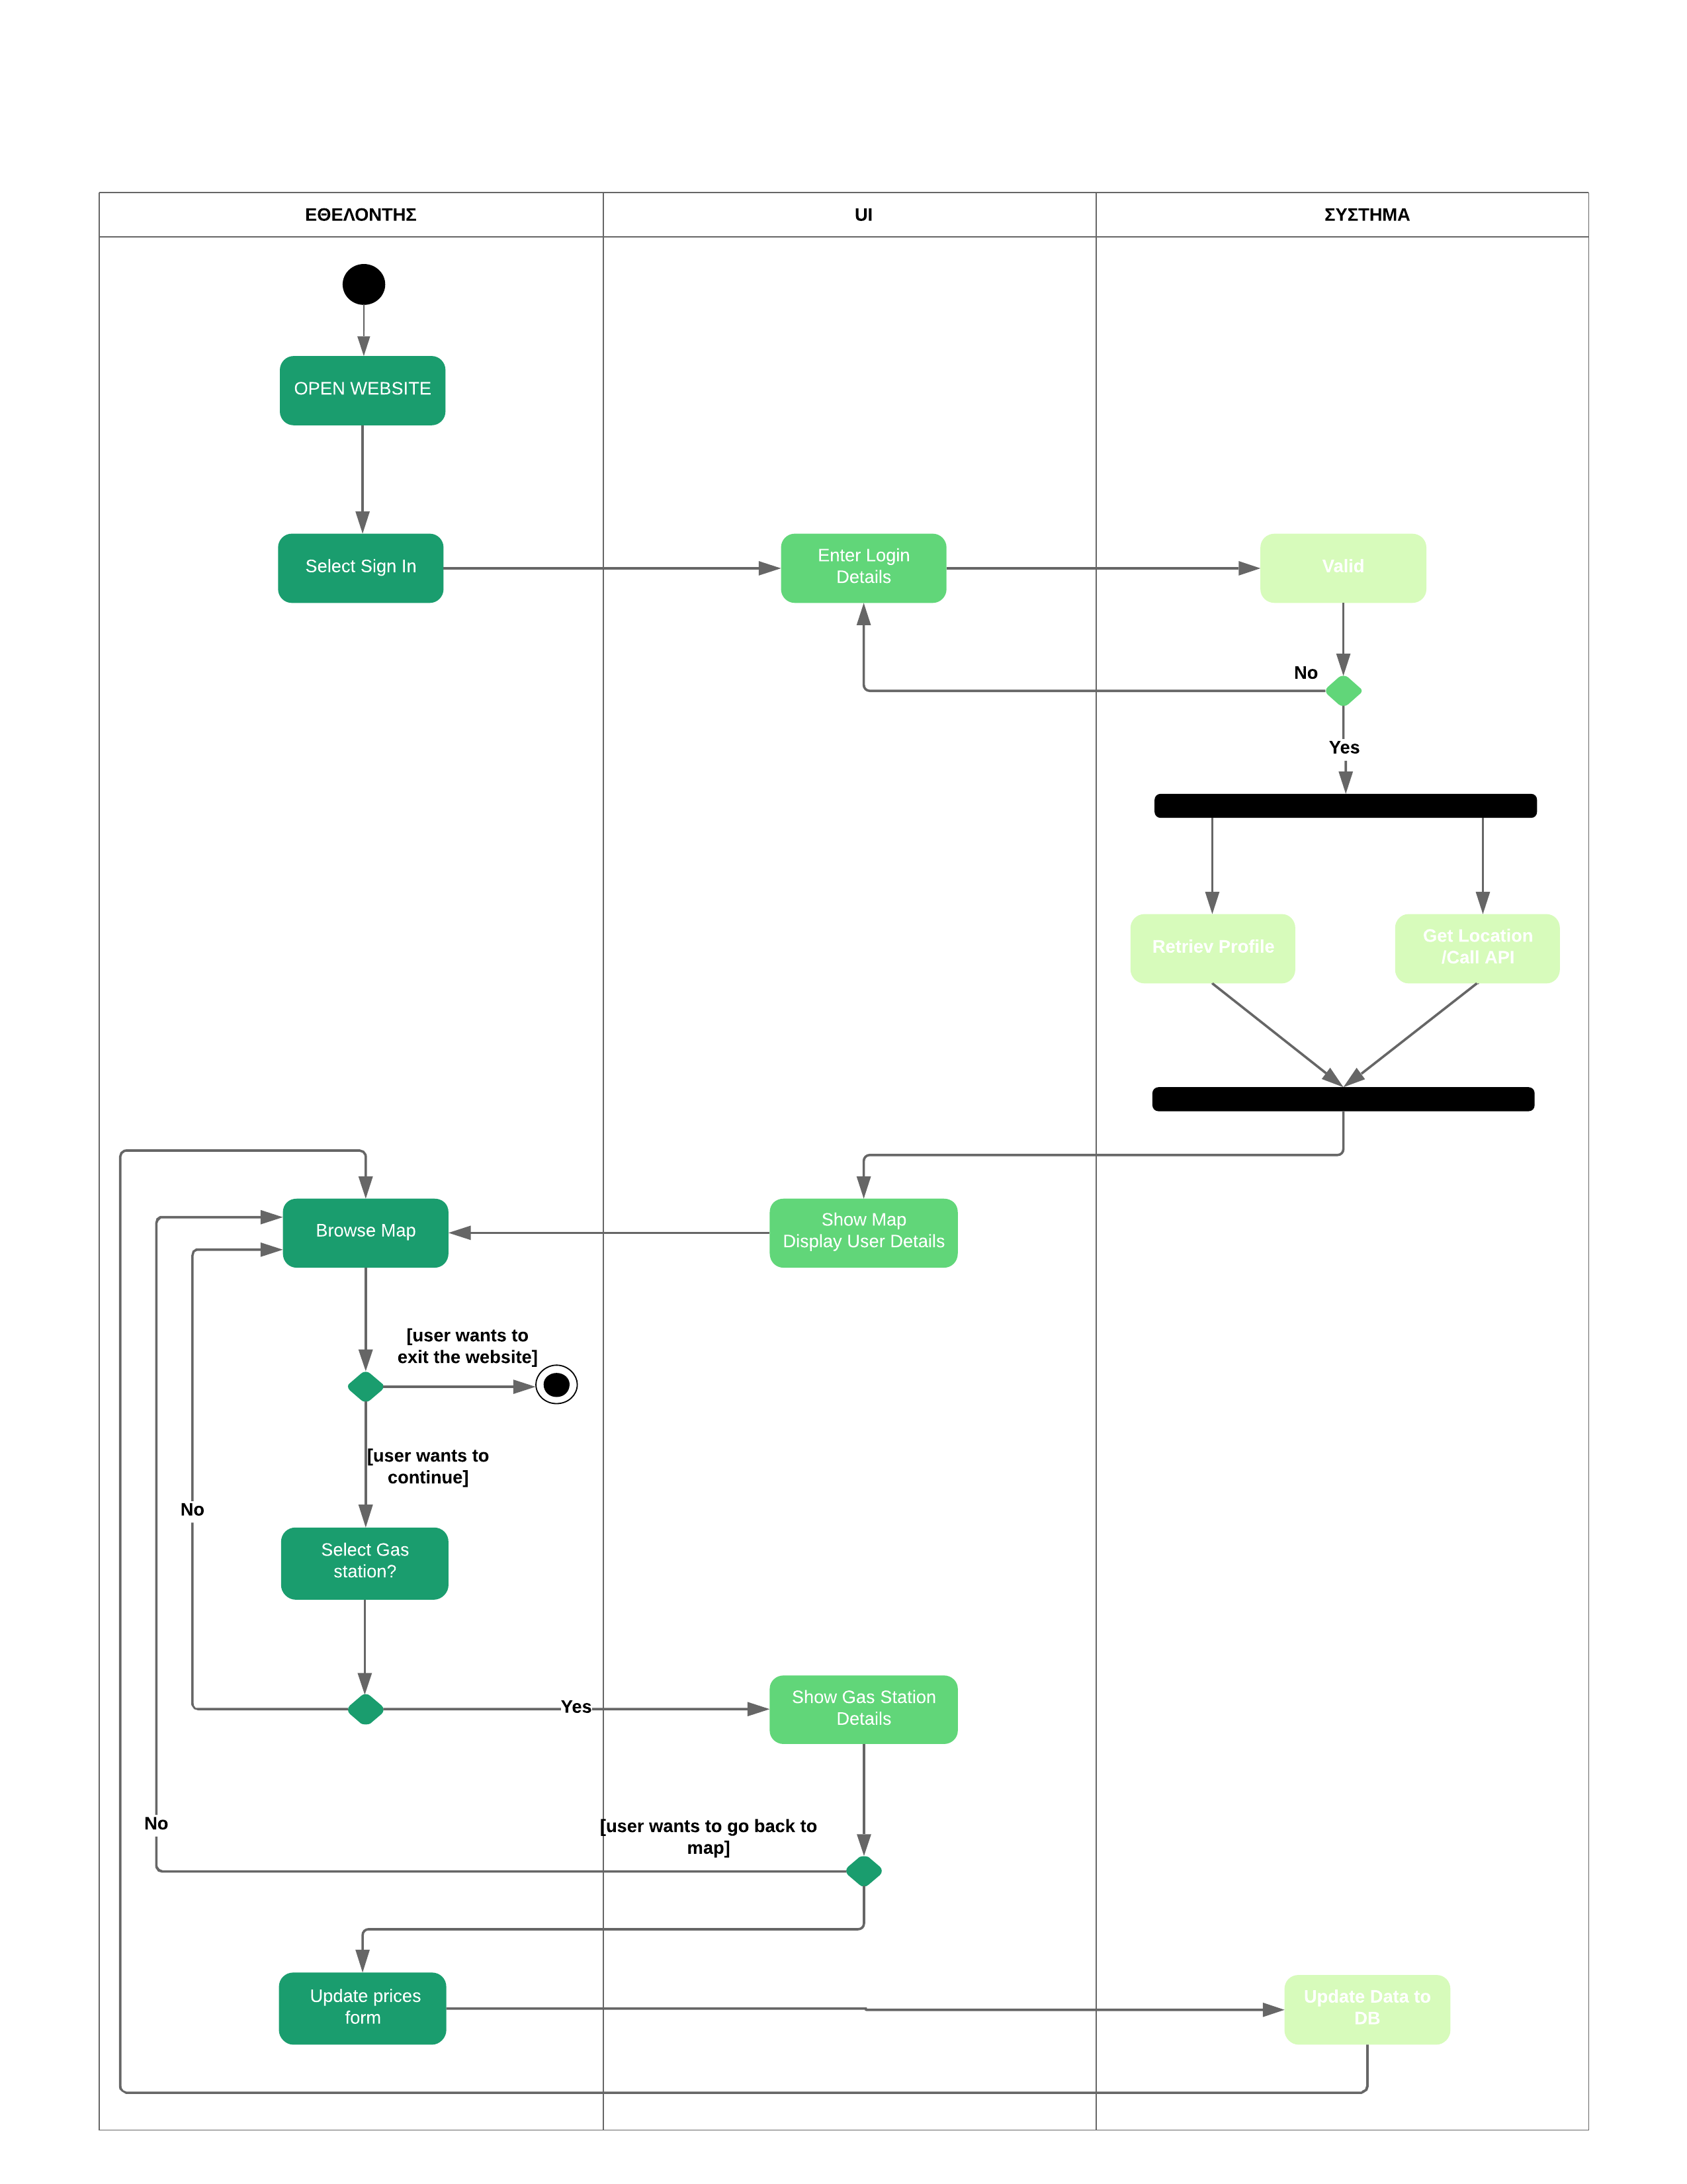
\includegraphics[width = \linewidth]{uml/volunteer.png}
	\caption{UML activity diagram για \texttt{ΕΘΕΛΟΝΤΗ} (εγγεγραμένος χρήστης-ταυτίζεται για ιδιοκτήτη πρατηρίου υγρών καυσίμων)}
\end{figure}